\documentclass[journal,10pt,twocolumn]{article}
\usepackage{graphicx}
\usepackage[margin=0.5in]{geometry}
\usepackage[cmex10]{amsmath}
\usepackage{array}
\usepackage{booktabs}
\usepackage{mathtools}
\title{\textbf{Optimization Assignment - 1}}
\author{Akana Sai Kumar}
\date{Oct 2022}


\providecommand{\norm}[1]{\left\lVert#1\right\rVert}
\providecommand{\abs}[1]{\left\vert#1\right\vert}
\let\vec\mathbf
\newcommand{\myvec}[1]{\ensuremath{\begin{pmatrix}#1\end{pmatrix}}}
\newcommand{\mydet}[1]{\ensuremath{\begin{vmatrix}#1\end{vmatrix}}}
\providecommand{\brak}[1]{\ensuremath{\left(#1\right)}}
\providecommand{\lbrak}[1]{\ensuremath{\left(#1\right.}}
\providecommand{\rbrak}[1]{\ensuremath{\left.#1\right)}}
\providecommand{\sbrak}[1]{\ensuremath{{}\left[#1\right]}}

\begin{document}

\maketitle
\paragraph{\textit{Problem Statement} - A fruit grower can use two types of fertilizer in his garden, brand P and brand Q.The amounts (in kg) of nitrogen, phosphoric acid, potash, and chlorine in a bag of each brand are given in the table. Tests indicate that the garden needs at least 240 kg of phosphoric acid, at least 270 kg of potash and at most 310 kg of chlorine.\\
If the grower wants to minimise the amount of nitrogen added to the garden, how many bags of each brand should be used? What is the minimum amount of nitrogen added in the garden?} 
\vspace{1mm}
\begin{tabular}{|c|c|c|}
\hline
 Kg per bag & Brand P& Brand Q  \\ 
 \hline
 Nitrogen & 3 & 3.5 \\  
 \hline
 Phosphoric acid & 1  & 2 \\
 \hline
  Potash & 3 & 1.5 \\
 \hline
 Chlorine & 1.5 & 2\\
 \hline
\end{tabular} \\



\section*{\large Solution}
Let x be the bags of Brand P, y be  the bags of Brand Q. The problem can be formulated as
\begin{align}
	P = \min_{x,y} \vec{x}\\
	2x + y \geq 180\\
	x + 2y \geq 240\\
	1.5x + 2y \leq 310\\
	x \geq 0\\
	y \geq 0
\end{align}
which can be expressed in vector form as
\begin{align}
	P = \min_{\vec{x}}\myvec{3&3.5}\vec{x}\\
	\myvec{2&1\\1&2\\-1.5&-2\\1&0\\0&1}\vec{x} = \myvec{180\\240\\-310\\0\\0}\\
	\vec{x} \geq \vec{0}
\end{align}
Solving using cvxpy, we get
\begin{align}
	P_{min} = 470\\
	\vec{x} = \myvec{40\\100}
\end{align}
Ploting
\centering{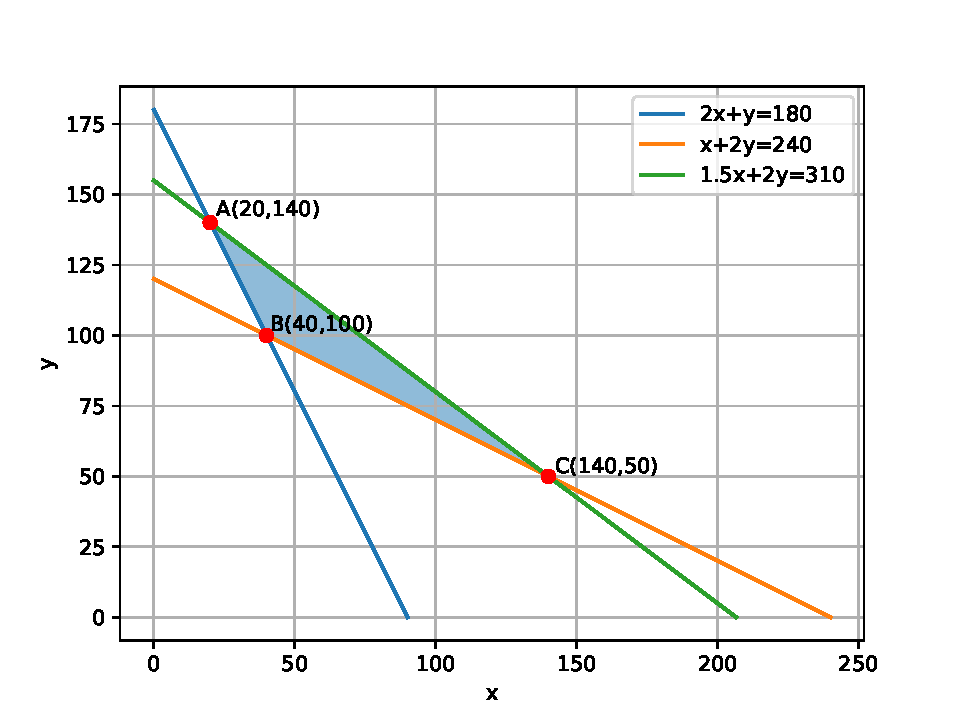
\includegraphics[scale=0.5]{op.pdf}}
\end{document}
